\section{The Generator}\label{generator}

The Generator tool is a graphical user interface developed in Java, allowing the user to store data from OWL files into a MySQL database. This tool also permits the user to query the database using the C++ function calls. The tool Generator is composed of the following functionalities:
\begin{enumerate}
 \item Convert OWL documents into SQL syntaxes (OWL to SQL).
 \item Translate SQL syntaxes to OWL language in order to modify an OWL document (SQL to OWL).
 \item Convert the OWL language into C++ classes (OWL to C++).
\end{enumerate}

To date, only steps 1. and 3. have been implemented and will be covered in this document.

\subsection{Prequisites}\label{s:prequisites}
The description of the Generator tool is given for a Ubuntu Linux system. To run and use the Generator tool, different applications must be installed on the system.

\subsubsection{Java Runtime Environment}
The Generator tool comes as a jar file. As such, the Java Runtime Environment should be installed on your system. This application can be found at \url{www.oracle.com}.

\subsubsection{MySQL Server and Client}
The MySQL server and client should be installed and running on your system.
\begin{itemize}
 \item \textit{sudo apt-get update} (Update the package management tools)
 \item \textit{sudo apt-get dist-upgrade} (Install the latest software)
 \item \textit{sudo apt-get install mysql-server mysql-client} (Install the MySQL server and client packages). You will be asked to enter a password.
\end{itemize}

When done, you have a MySQL database ready to run. The following command will allow you to run MySQL.

\begin{itemize}
 \item \textit{mysql -u root -p}
 \item Enter the same password you used when you installed MySQL.
\end{itemize}

Finally, we need the plugin \texttt{libmysqlcppconn-dev} which allows C++ to connect to MySQL databases. It can be installed as follows:
\begin{itemize}
 \item \textit{sudo apt-get install libmysqlcppconn-dev}
\end{itemize}

\subsection{How to Run the Generator Tool}\label{s:run}
The Generator tool can be launched using either one of these two following methods:
\begin{enumerate}
 \item \textit{java -jar Generator.jar}
 \item Right-click on Generator.jar and select the option ``Open With OpenJDK Java 6 Runtime". Note that this message will be different for future releases of the Java Runtime Environment.
\end{enumerate}


\subsection{Functionalities}\label{s:generator}
As mentioned in the Introduction, we are covering only steps 1. and 3. in the rest of this document, i.e., \textit{OWL to SQL} and \textit{OWL to C++}, respectively.

\subsubsection{OWL to SQL}
\begin{figure}[h!t!]
\centering
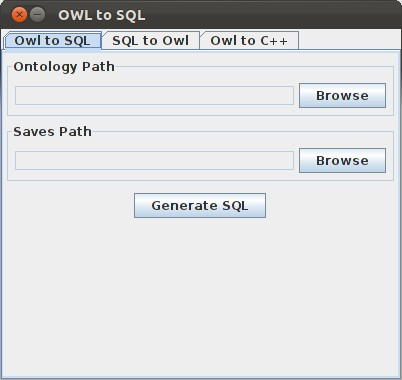
\includegraphics[width=9cm]{Figure/OWLtoSQL001.jpeg}
\caption{Owl to SQL tab.}
\label{fig:owl2sql}
\end{figure}
To convert OWL classes and instances to SQL, the \texttt{Owl to SQL} tab should be selected (see Figure~\ref{fig:owl2sql}). The different fields are:

\paragraph{Generate SQL Files}
\begin{itemize}
 \item Ontology Path: This field requires the file \texttt{kittingInstances.owl}. Before doing so, you need to modify one line in this file. Open it with a text editor and find the line \texttt{Import(<file:kittingClasses.owl>)}. Modify
this line by giving the absolute path to the file \texttt{kittingClasses.owl}. You should should have something that looks like \texttt{Import(<file:/home/username/NIST/ipmas/Generator/kittingClasses.owl>)}. When this is done, save the file, and browse to  \texttt{kittingInstances.owl} using the ``Browse" button.
 \item Browse to the directory where you want to save the SQL files.
\end{itemize}

Once the two previous steps are done, click on ``Generate SQL''. You should receive a message confirming the generation of the SQL files: \texttt{kittingInstances.owlCreateTable.sql} and \texttt{kittingInstances.owlInsertInto.sql}. The former is used to create tables, the latter is used to populate these tables;

\paragraph{SQL Tables and Insertions}
The next step is to create a database and to populate it.

\begin{itemize}
\item Connect to mysql using \textit{mysql -u root -p}, then enter your password. You should be in the mysql shell if this succeeded (\textit{mysql>}).
\item Delete a previous database (if you already used this tool and you want to replace the existing database with this new one) :
\texttt{mysql>} \textit{DROP DATABASE OWL;} (\textit{OWL} is the name of the old database).
\item Create a database:
\begin{itemize}
\item \texttt{mysql>} \textit{CREATE DATABASE OWL;}. Here, \textit{OWL} is the name of the database (you can use a name of your choice).
\item Before performing the following commands, we need to tell MySQL which database we are planning to work with (\textit{OWL} in our case). This is done using:
\begin{itemize}
\item[] \texttt{mysql>} \textit{USE OWL}
\end{itemize}
\end{itemize}
\item Populate the database with tables using \texttt{kittingInstances.owlCreateTable.sql}.
\begin{itemize}
 \item \texttt{mysql>} \textit{source <path>/kittingInstances.owlCreateTable.sql;}
\end{itemize}

\item Populate the tables with data using \texttt{kittingInstances.owlInsertInto.sql}:
\begin{itemize}
 \item \texttt{mysql>} \textit{source <path>/kittingInstances.owlInsertInto.sql;}
\end{itemize}
\end{itemize}

\textit{<path>} designs the absolute path to the appropriate file.

\subsubsection{OWL to C++}
\begin{figure}[h!t!]
\centering
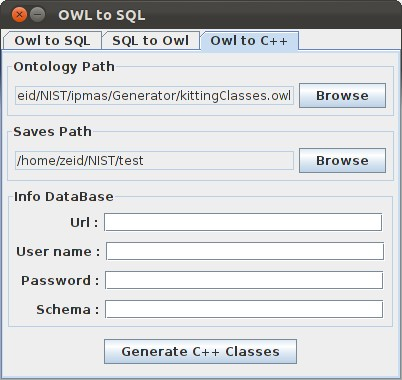
\includegraphics[width=9cm]{Figure/OWL2C++.jpeg}
\caption{Owl to C++ tab.}
\label{fig:owl2C++}
\end{figure}
The ``Owl to C++" tab (see Figure~\ref{fig:owl2C++}) is used to generate C++ classes and scripts allowing the connection between C++ and MySQL. The different fields are explained below:
\begin{itemize}
\item \textbf{Ontology Path}: This is the path to the ontology (\texttt{kittingClasses.owl} in our example).
\item \textbf{Saves Path}: Directory where the C++ files and scripts will be generated.
\item \textbf{Url}: This is the url of the database. It's usually the IP address of the machine hosting the database (127.0.0.1 if it is local).
\item \textbf{User name}: User name used to connect to the MySQL database.
\item \textbf{Password}: Password associated to the user name to connect to the MySQL database.
\item \textbf{Schema}: This is the name of the database (\textit{OWL} in our example).
\end{itemize}

When all the fields are completed, click the ``Generate C++ Classes" button to generate C++ and script files.